\section{Implementation}
\label{cha:implementation}
% TODO: Insert previous chapter references
This chapter details the technical implementation of the concepts introduced in the previous section. While the Approach chapter established the conceptual and algorithmic foundations of the proposed scheduling framework, the following sections focus on how these ideas were realized in practice. The implementation emphasizes architectural modularity, clear component interfaces, and the integration of machine learning-based decision layers within a simulation-driven environment. Each subsystem—from the monitoring client and statistical modeling backend to the simulation environment—was designed to remain functionally independent while communicating through well-defined data and control flows. This decoupled design not only facilitates reproducibility and maintainability but also enables future extensions, such as the replacement of predictive models or the addition of new scheduling policies, without major structural changes. The remainder of this chapter outlines the overall system architecture, mentions the chosen technologies and design principles, and describes the concrete implementation of the monitoring client, the statistical learning components, and the simulator setup.

\subsection{System Architecture}
\label{sec:system_architecture}
% Overview sketch


\subsection{Technology and Design Choices}
\label{sec:technology_and_design_choices}
% Provide a table per number of the previous figure with the technology and design choice and a brief justification.
\begin{figure}[H]
    \centering
    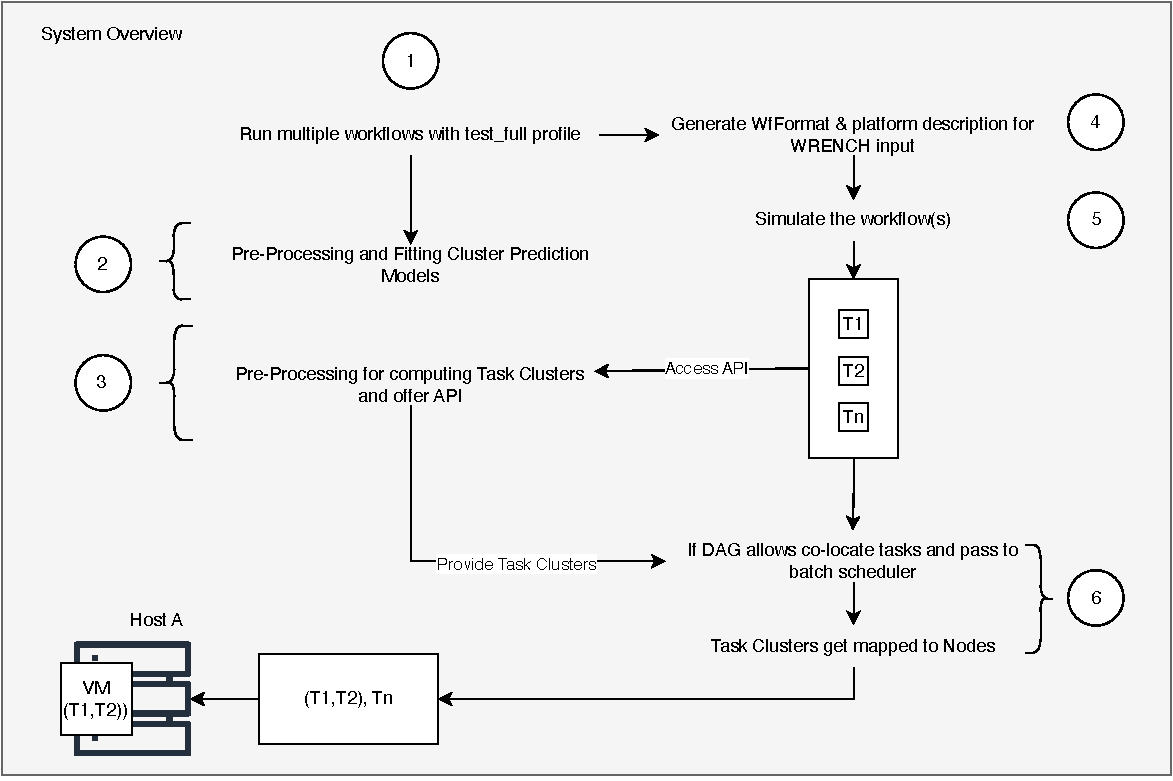
\includegraphics[scale=0.7]{fig/05/05-system-overview.pdf}
    \caption{System Overview}
    \small
    \label{fig:05-system-overview}
    \tiny
    A Scientific Workflow Task as part of a Workflow consuming input data and producing output data.
\end{figure}
% TODO: It shadows the page number
\begin{table}[H]
    \centering
    \caption{Monitoring features and associated technical components.}
    \label{tab:monitoring_layers}
    % ↓↓↓ kleinere Schrift + etwas engerer Zeilenabstand ↓↓↓
    \small
    \renewcommand{\arraystretch}{1.05}
    \resizebox{\textwidth}{!}{
        \begin{tabular}{
            p{4.5cm}
            >{\centering\arraybackslash}p{2.8cm}
            p{8.2cm}
        }
            \toprule
            \textbf{Component Category} & \textbf{Software Used} & \textbf{Comments / Functionality} \\
            \midrule

            \multicolumn{3}{l}{\textbf{Workflow Execution}} \\[3pt]
            Operating System & Ubuntu 22.04.5 LTS & Base system environment for all components. \\
            Kernel & Linux 5.15.0-143-generic & Provides low-level system resource management. \\
            Workflow Management Engine & Nextflow 25.06.0 & Controls workflow DAG execution and task dependency resolution. \\
            Virtualization Layer & Docker Engine 28.3.1 (Community) & Provides isolated VM environments for task execution. \\
            Resource Manager & Slurm 24.05.2 & Allocates CPU and memory resources dynamically across hosts. \\

            \midrule
            \multicolumn{3}{l}{\textbf{Monitoring System}} \\[3pt]
            Time-Series Database & Prometheus Server 3.3.1 & Central metric collector and time-series database. \\
            Monitoring Client & Go 1.24.1 & Collects per-node and per-container resource metrics. \\

            \midrule
            \multicolumn{3}{l}{\textbf{Workload Experiments}} \\[3pt]
            Benchmark Execution & stress-ng 0.13.12 & Generates controlled CPU, memory, and I/O workloads. \\
            Monitoring & Deep-Mon (custom fork) with Python 3.10.12 \& BCC 0.35.0 & Captures resource traces during workload execution. \\

            \midrule
            \multicolumn{3}{l}{\textbf{Data Analysis}} \\[3pt]
            Feature Engineering & Jupyter Kernel 6.29.5, Python 3.10.12, Poetry 2.1.2 & Derives and normalizes temporal task signatures. \\
            Clustering & scikit-learn 1.5.2 & Groups similar task behaviors into consolidated classes. \\
            KCCA & CCA-Zoo 2.5.0 & Learns correlations between performance and energy domains. \\
            Random Forest Regressor & scikit-learn 1.5.2 & Predicts runtime and power consumption from task signatures. \\
            Kernel Ridge Regression & scikit-learn 1.5.2 & Baseline model for non-linear regression comparison. \\

            \midrule
            \multicolumn{3}{l}{\textbf{Simulation Framework}} \\[3pt]
            Workflow Tracing & Nextflow Tracer (custom fork) & Records execution-level metadata for simulation replay. \\
            Simulation Engine & WRENCH 2.7 \& C++17 & Evaluates scheduling strategies under controlled conditions. \\
            Clustering API & FastAPI 0.1.0, Python 3.10.12 & Provides task grouping via \textit{ShaReComp} integration. \\
            Prediction API & FastAPI 0.1.0, Python 3.10.12 & Interfaces learned models for runtime and energy estimation. \\

            \bottomrule
        \end{tabular}
    }
\end{table}


\subsection{Decoupled Design for further Research}
\label{sec:extensibility_through_decoupled_design}
The extensibility of the overall system is achieved through a decoupled design that separates monitoring, modeling, and simulation components while maintaining clear communication interfaces between them. Each part of the system can evolve independently without impacting others, enabling modular experimentation with new data sources, predictive models, or scheduling strategies. This modularity supports reproducibility and future extensibility, as new data collection layers or simulation backends can be added by extending interfaces rather than rewriting existing code.

\subsubsection{Configurable Monitoring Client}
\label{sec:monitoring_client}
The monitoring client exemplifies this philosophy by relying on a flexible configuration-driven architecture. Using a YAML-based configuration file, it dynamically defines which metrics to collect from heterogeneous data sources such as Prometheus exporters, cAdvisor, eBPF probes, or SNMP-based sensors. The configuration specifies not only the metric names and queries but also the identifiers and units, allowing seamless adaptation to different environments or workflow engines. This separation of logic and configuration enables the same client to operate across diverse infrastructures without recompilation. The clients implementation, built on the Prometheus API, abstracts away the complexity of time-range queries and concurrent metric fetching through lightweight threading and synchronization mechanisms. As a result, developers can extend the monitoring framework simply by adding new data sources or metrics to the configuration file, without altering the underlying collection logic.

% Config File
\lstinputlisting[
    language=YAML,
    caption={Example YAML Configuration File},
    label={lst:yaml_config}
]{/home/nfomin3/dev/ThesisDocument/fig/05/05-pcm-config.yml}

\verbfilenobox[\mbox{\scriptsize\theVerbboxLineNo:}]{fig/05/05-pcm-config.yml}

\subsubsection{Enabling Access to Co-location Hints in the Simulator}
\label{sec:statistical_modeling}
The statistical modeling component, implemented as a standalone FastAPI service, follows a similar modular design. It exposes a clean, language-agnostic HTTP API that separates the inference logic from data ingestion and model management. The service maintains state for clustering and prediction requests, delegating core computational tasks to dedicated helper functions. This decoupling makes it straightforward to replace or add new predictive models, such as neural architectures or alternative regression approaches, without modifying the API contract. The clustering and prediction endpoints can interact with any external workflow manager or simulator via standardized JSON payloads, ensuring flexibility in integrating new pipelines or retraining procedures. This independence between model serving and data processing pipelines also simplifies scalability, allowing the modeling service to be containerized and deployed independently for distributed or cloud-based setups.

% Graphic with API Endpoints showing the implemented capabilities:

\begin{table}[H]
    \centering
    \caption{Overview of REST API Endpoints Exposed by the \textit{ShaReComp} Service.}
    \label{tab:api_endpoints}
    \renewcommand{\arraystretch}{1.15}
    \resizebox{\textwidth}{!}{
        \begin{tabular}{
            p{0.8cm}
            p{5.3cm}
            >{\centering\arraybackslash}p{2cm}
            p{9cm}
            }
            \toprule
            \textbf{\#} & \textbf{Endpoint}               & \textbf{Method} & \textbf{Description / Response Schema}                   \\
            \midrule

            1           & \texttt{/clusterize\_jobs}      & POST            &
            Clusters nf-core jobs based on historical data. \newline
            \textit{Request:} \texttt{ClusterizeJobsRequest} (list of job names). \newline
            \textit{Response:} \texttt{ClusterizeJobsResponse} (cluster mapping with run ID).                                          \\

            2           & \texttt{/predict}               & POST            &
            Predicts runtime and power consumption for consolidated job clusters. \newline
            \textit{Request:} \texttt{PredictRequest} (cluster IDs, model types). \newline
            \textit{Response:} \texttt{PredictionResponse} (predicted values for each model).                                          \\

            \midrule
            \multicolumn{4}{l}{\textbf{Component Schemas}}                                                                             \\[3pt]

            --          & \texttt{ClusterizeJobsRequest}  & Object          &
            \textbf{Fields:} \texttt{job\_names} (array of strings). Required.                                                         \\

            --          & \texttt{ClusterizeJobsResponse} & Object          &
            \textbf{Fields:} \texttt{run\_id} (string), \texttt{clusters} (map of arrays). Required.                                   \\

            --          & \texttt{PredictRequest}         & Object          &
            \textbf{Fields:} \texttt{cluster\_ids} (array), \texttt{prediction\_models} (array of \texttt{PredictionModel}). Required. \\

            --          & \texttt{PredictionModel}        & Object          &
            \textbf{Fields:} \texttt{model\_type} (array of strings). Required.                                                        \\

            --          & \texttt{PredictionResponse}     & Object          &
            \textbf{Fields:} \texttt{run\_id} (string), \texttt{predictions} (nested map of numeric values). Required.                 \\


            \bottomrule
        \end{tabular}
    }
\end{table}

\subsubsection{Used Simulator Components}
\label{sec:simulator_setup}
The simulator setup further demonstrates the benefits of this decoupled design. The resource management layer of the simulator exposes generic interfaces for allocators, schedulers, and node assigners, allowing any of them to be replaced or combined dynamically at runtime. This separation allows the same simulator to execute both baseline and experimental resource allocation strategies without modifying the controller logic. Through this design, the simulator can execute diverse workflow types by merely switching configuration parameters or class bindings. Moreover, the integration of energy and performance tracing through independent services ensures that extending the simulator with new measurement capabilities does not interfere with the scheduling or execution logic.

% Show cpp code of base directory
\lstinputlisting[
    language=C++,
    caption={WRENCH C++ Simulation File},
    label={lst:cpp_sim},
    basicstyle=\ttfamily\footnotesize,
    keywordstyle=\color{blue},
    commentstyle=\color{gray},
    stringstyle=\color{red},
    numbers=left,
    numberstyle=\tiny,
    stepnumber=1,
    numbersep=5pt,
    breaklines=true,
    frame=single
]{/home/nfomin3/dev/ThesisDocument/fig/05/05-wrench-sim.cpp}